%!TEX root = paper.tex
\section{Introduction}
Programming networks to correctly forward flows according to user- and
application-induced policies is difficult and
error-prone~\cite{troubleshooting, bgpmisconfig}. 
At least three
common characteristics of network policies are to blame: (1) A network
may need to satisfy several types of policies, including reachability
(i.e., which endpoints can communicate), isolation (i.e., which flows
cannot share links), service chaining (i.e., which ``middleboxes'',
e.g., firewalls or load balancers, must be traversed), resilience
(e.g., number of available backup paths), and traffic engineering
(e.g., minimizing average link utilization). (2) The network must
provide certain guarantees in the event of failures. Ideally, every
set of forwarding paths (i.e., data plane) installed in the network
should conform to the above policies, otherwise performance, security, or
availability problems may arise. (3) Most policies are global---i.e.,
they concern end-to-end paths, not individual devices/links.

The global nature of network policies is one motivation for
software-defined networking (SDN). SDN allows paths to be centrally
computed over a global view of the network. However, ensuring paths
are correctly computed and installed in the presence of failures is
difficult in practice, even if the SDN controller is
distributed~\cite{hasdn}.  Traditional control planes rely on
distributed protocols such as Open Shortest Path First (OSPF) and
Border Gateway Protocol (BGP) to compute paths; these protocols
typically employ variants of least cost path computation, and react to
failures by recomputing least cost paths and installing forwarding
state in routers that induces the paths. In contrast to centralized
SDN, traditional control planes offer greater fault tolerance; but,
determining the appropriate distributed realization of policies is
hard~\cite{propane}.

Our high-level goal is to develop a system to {\em automate the
  process of creating a correct and failure-resilient distributed
  realization of policies in a traditional control plane}. To be
useful, such a system must satisfy a few key requirements. (1) It must
handle a wide range of commonly-used policies---including
reachability, service chaining, and traffic engineering---to meet
applications' diverse security and compliance requirements. (2) It
must ensure that configurations are resilient to network malfunctions
such as link failures. (3) It must provide support for realizing
hierarchical control planes--- where a network is split into several
``domains'' atop which a hierarchy of intra- and inter-domain control
plane configurations is deployed---to ensure scalability for large
networks~\cite{routingdesign}. (4) To improve manageability and
network cost-effectiveness~\cite{mpa-imc15,complexity:sigcomm11}, it
must ensure that configurations obey certain general
rules-of-thumb~\cite{complexity:nsdi09}, e.g., limiting the number of
lines of configurations and the use of certain configuration
constructs.

Thus, our work contrasts with prior efforts which suffer
from one or more drawbacks: they generate SDN- or BGP-specific
control planes for a limited range of policies (e.g., peering)
~\cite{netkat,merlin,netegg,fattire,simple,sol,propane}; do not
attempt to be resilient to failures~\cite{synet}; 
do not support generating
hierarchical control planes~\cite{propane}; 
and do not enable generation of
simple-to-manage network configurations. 

The problem of synthesizing router configurations for which the
distributed control plane is resilient to failures and generates
policy-compliant paths is computationally hard. Even generating a set
of policy-compliant paths for an SDN is computationally hard---e.g.,
enforcing isolated paths is NP-complete. While it is possible to
develop algorithms for individual policies, accommodating multiple
policies and the above requirements is extremely difficult.


An attractive possibility, motivated by recent progress in program
synthesis, is to use
%% By bringing ideas from program synthesis approaches, one could try to 
%% synthesize configurations using 
Satisfiability Modulo Theories (SMT) solvers to automatically search
the space of distributed configurations for a suitable ``solution'' --
i.e., concrete router configurations that satisfy input policies and
the aforementioned four requirements. SMT solvers provide support for
constraint solving for propositional logic (SAT) and linear rational
arithmetic (LRA); these powerful theories can  
encode properties on network paths 
and configurations. Thus, an SMT-search based approach can, in theory,
provide support for multiple policies and different manageability requirements. 
This approach also decouples the requirements from the underlying search, 
and thus, could be extended to support new policies. 

However, using SMT solvers in our context is
non-trivial.  To infer the concrete set of paths induced by network
configurations, one has to incorporate into synthesis complex
concepts---e.g., reasoning about shortest path algorithms requires
constraints in complex theories (SAT and LRA).  Even with recent
advances in SMT solving, approaches that directly generate
configurations from policies do not scale to moderately-sized networks
or sets of policies~\cite{synet}. Furthermore, generating resilient
control planes needs reasoning about how protocols react to failures,
which further complicates an already intractable synthesis
problem. Control plane hierarchy and manageability requirements further
complicate the problem.

\begin{figure}
	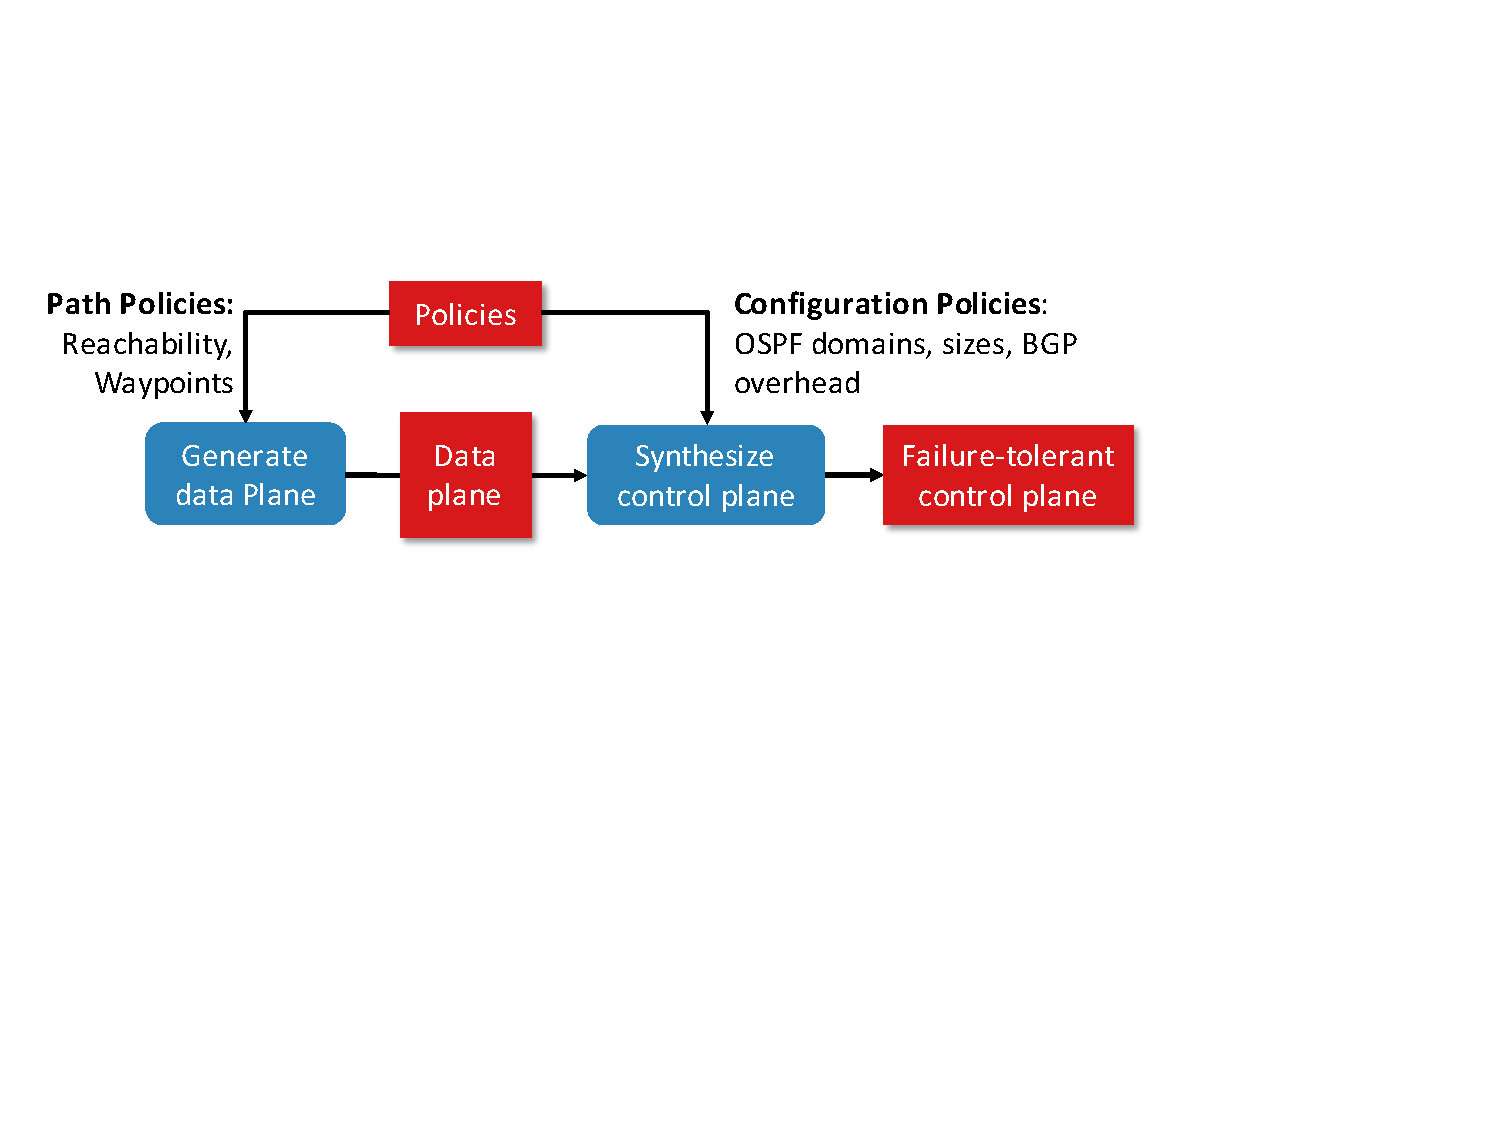
\includegraphics[width=\columnwidth]{figures/architecture.pdf}
	\compactcaption{Two-phase process for generating a control plane
		with failure-tolerance properties}
	\label{fig:architecture}
\end{figure}

In this paper, we present \name, a system that overcomes the above
challenges in SMT-based distributed configuration synthesis.  \name
uses a two-phased approach for tractability (\Cref{fig:architecture})
that does not attempt to generate a policy-compliant control plane in
a single step.  First, \name uses \genesis~\cite{genesis} to
synthesize paths---i.e., the network forwarding state---that are
compliant with given policies, such as, waypoints and isolation.
\name then generates intra-domain (shortest-path OSPF) and
inter-domain (BGP) router configurations that induce the forwarding
state synthesized by \genesis\ {\em and} provide high resilience. \name 
is catered for moderate-sized enterprises and multi-tenant datacenters 
which require support for diverse policies.

We consider three settings with progressively more complex policies
and resilience requirements and show how \name, using its two-phase
approach, can effectively generate highly-resilient and
policy-compliant solutions.

First, we consider a setting in which the operator of a hierarchically
structured network wants to enforce a large diverse set of complex
policies (waypoint traversal, isolation, traffic engineering, etc).
The operator also requires a simple notion of
\emph{connectivity-resilience} to guarantee that, under most common
link failures, packets can still reach their destination.  In this
case, \name synthesizes OSPF configurations using linear constraint
solving to compute link weights, and uses the unsatisfiable cores of
failed solving attempts to judiciously place a small number of static
routes.  \name synthesizes BGP configurations directly from the domain
mapping (i.e., which router belongs to what domain) and the paths.
Using these techniques, \name can generate configurations that are
$10\%$ more resilient than configurations that only use static routes.

Second, we consider a setting in which the operator wants to guarantee
that, for common link failures, the resulting configuration is
policy-compliant.  We call this notion \emph{policy-resilience}.
Since synthesizing policy-resilient configuration is very difficult in
the general case, we focus on a {\rm restricted class} of policies:
for traffic class (src-dst subnet pair), we allow the operator to
specify a set of waypoints that packets must traverse before reaching
their destination.  We modify our linear constraints to guarantee that
at least two paths that traverse the waypoints have path cost (e.g.,
OSPF path cost) lower than any path not going through a waypoint, thus
providing 1-resilience under failure. Using this, \name can generate
configurations that are $140\%$ more policy-resilient than
configurations generated with our first technique.

Finally, we consider a setting where the operator can specify bounds
on the number and sizes of domains her control plane is organized
into, and the ability to assign routers to different domains.  We
present a stochastic search technique that leverages this flexibility
to look for ways to assign routers to different domains so that the
synthesized configurations have even higher resilience.  Through this,
\name can further improve the resilience of the configurations by
$10\%$. We show that \name can be naturally used to bound or optimize
different configuration metrics such as static routes and BGP
configurations' size to improve network manageability.

Our experiments show that, thanks to its two-phase approach, \name can
synthesize connectivity-resilient configurations for medium-sized
datacenter topologies in $< 10$ {\em minutes} and policy-resilient configurations
in under an hour.  Notably, \name's performance is {\em 2-3 orders of
  magnitude} faster than the state-of-art network configuration
synthesis system SyNET~\cite{synet}, which uses a direct synthesis
approach based on SMT.

\minisection{Contributions} We make the following contributions.
\begin{itemize}	
    \item \name, a framework for
	that enforces policies in ``traditional'' (OSPF and BGP) networks
	by synthesizing highly-resilient router configurations. 		
	\name  uses concrete
	paths to guide the synthesis  
	instead of directly generating policy-compliant
	configurations.

	\item An algorithm for synthesizing policy-compliant
          configurations with few statically assigned routes. This
          algorithm yields configurations with high network
          connectivity even in the presence of link failures
          (\S~\ref{sec:config-synthesis}).

	\item An algorithm for synthesizing policy-compliant 		
		 configurations that is specialized for waypoint policies. 
		 This algorithm yields configurations that have
		 high policy compliance even in the presence of link failures (\S~\ref{sec:ospfwaypoint}). 
	
	\item A stochastic search mechanism for finding 
		partitions of the network into multiple routing domains which
		yield configurations with higher resilience (\S~\ref{sec:synth-dom-ass}).
	
	\item An implementation of \name together with an evaluation
          of its algorithms for different workloads, and comparison with a state-of-the-art
          configuration synthesis tool (\S~\ref{sec:evaluation}).
\end{itemize}
